\documentclass{article}
\usepackage{tikz}
\usepackage[letterpaper,scale=0.8]{geometry}
\usepackage{graphicx}
\setlength\parindent{0pt}
\setlength\parskip{1em}

\title{PakMan: A personal Package Manager}
\author{Zixi Li,\\ Instructor: Thomas Moon}

\begin{document}
\maketitle
\par \textbf{Abstract} This article described the design and implementation of a package manager that is designed to be cheap and expandable. The system is targeting families that live in private houses and want a cheap upgrade to their mailbox. Each package will be assigned a cabinet for storage when the owner is away, and the owner can retrieve the packages when he comes back. Comparing to existing solutions like Amazon lockers and UPS lockers, this system can be set up by the user himself. To cope with various needs, the user can choose to have any number of lockers in his system and add/remove lockers dynamically according to their needs.
\newpage
\section{Incentive}
\par Many American families live in private houses of a sparse neighborhood. With the ongoing trend of online shopping and cloud business, more and more orders are being processed online and delivered to your door. It is convenient to have your door opened and get the item you ordered right at your doorsteps -- except sometimes they don't. Packages, unless otherwise marked as important or require a signature, will be simply delivered at the porch where everyone can see it. There's no way to prevent someone from passing by and steal it. Even if you have a surveillance camera, it takes lots of time and effort to report the case to the police and there's little chance of getting your item back.

\par Solutions to this problem have been rolling out: UPS has lockers set at neighborhoods, and Amazon has staffed pick-up locations with lockers. However, these solutions are not universal, as they can only be used by said providers. Secondly, not everyone had the luck of living near such locations.

\par Therefore, I came up with an idea of a personal package locker - A locker that can be set at the door and used by the family. They do not need to have large storage capacity because they only serve one user. Also, it should come in pieces that can be easily assembled instead of large parts, so it will be easier for families to set them up.

\section{Design}
\par For the user interface, there should be the a panel with display and keyboard, and acts as the main panel of the locker. The delivery man can enter the package number and drop the package at the machine, and the user can retrieve the package by entering the password.

\par We want the system to be easy to assemble, so each cabinet should come individually, and the user should be able to add or remove cabinets on the go. Connecting each cabinet directly is not a great solution. Each cabinet will take up some pins on the controller so the design is not expandable, because the software have to be modified for each additional cabinet. To achieve an expandable architecture, I chose to have a separate controller for each cabinet that handles some functions like indicator lights and a button, and the main controller will communicate with the sub-controllers thorough a two-wire interface. The two-wire interface is a protocol that allows up to 256 devices to communicate with only two signal wires. Devices can be daisy-chained on the same line without additional configuration.

\par Since each cabinet is connected individually, it becomes possible for a daring thief to steal a single cabinet, with the content in it. Therefore, the main controller will have an alarm system that get triggered when a cabinet is missing. This can be done by scanning the bus periodically, and trigger the alarm if any cabinet is missing for a period of time.

\section{Main Controller}
\par The main controller is the heart of the whole system. It provides the interface between the system and the user, handles package delivery, system management functionalities, and passes down commands to the sub-controllers.

\subsection{MCU Selection}
\par For my design, I selected STM32F407VET from ST Electronics as the main controller. It's a feature-rich performance processor based on ARM architecture that offers lots of system resources. I clocked it at 96MHz. For the development toolchain, I used the official HAL library that handles basic functionalities like GPIO and communication protocols, with the official STM32CubeIDE (based on Eclipse).

\subsection{User Interface}
\par To display enough information and save cost, I chose a 20x4 matrix-dot character LCD for the central unit. The screen communicates with the main controller through a 4-bit parallel interface and some clock wires. The data transmission rate is low but adequate.

\par The keyboard is a 16-key matrix keyboard, with numbers and letters A,B,C,D. The letters are used as functions keys like "Accept" and "Cancel". Some glue logic is attached to the keyboard so an interrupt will be produced whenever a key is pressed, and the controller can scan the wires to find which key is being pressed.

\par Text and instructions will be shown on the display with multiple levels of menu. The user can easily navigate through the menu and choose his/her intended operation. To save energy, the controller will automatically return to idle and shutdown the screen backlight if no keyboard input was received for a period of time.

\subsection{Connectivity}
\par The most important hardware connectivity we're using on this device is the I2C interface. The processor have hardware I2C connectivity, which is configured to be an I2C master, driving a bus with the sub-controllers. The Physical data rate limitation on our setup is 1Mbps across all devices, but that's more than enough since the commands never exceed 2 bytes.

\par Besides that, a SPI interface is configured to communicate with a flash chip on the development board, which can be used to store permanent information. Another UART interface is configured to send debug data.

\section{Sub Controllers}
\par The sub-controllers have far less functions than the main controller, requiring less powerful hardware. I used Arduinos for the sub-controllers. Arduino Nano is compact yet still offer the connections we need, and any other Arduino more powerful than that can also do the job.

\par The sub-controller will have red and green lights, indicating whether the current cabinet is occupied. There's also a button for the delivery man to choose cabinets. All the sub controllers run on 4 common wires: two for power, two for communication. Connections are illustrated as in Figure 1.

\begin{figure}
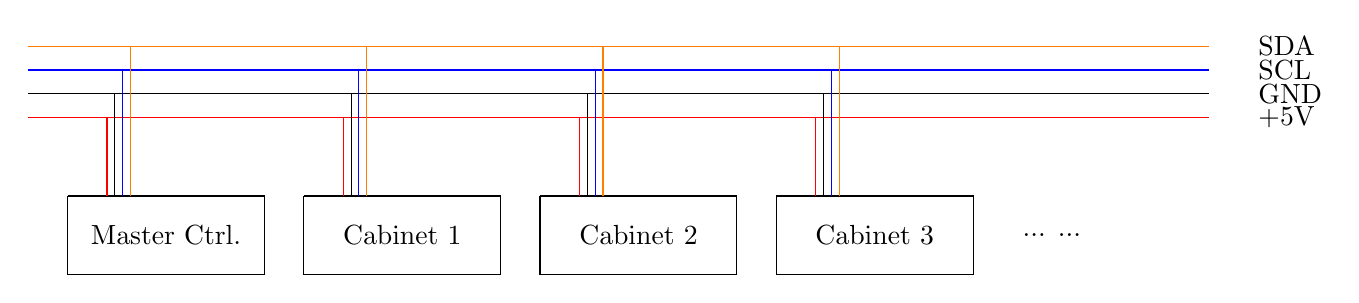
\begin{tikzpicture}
\draw [red] (0,0) -- (15,0);
\draw [black] (0,0.3) -- (15,0.3);
\draw [blue] (0,0.6) -- (15,0.6);
\draw [orange] (0,0.9) -- (15,0.9);
\node [right] at (15.5,0) {+5V};
\node [right] at (15.5,0.3) {GND};
\node [right] at (15.5,0.6) {SCL};
\node [right] at (15.5,0.9) {SDA};

\draw (0.5,-1) -- (3,-1) -- (3,-2) -- (0.5,-2) -- (0.5,-1);
\node at (1.75,-1.5) {Master Ctrl.};
\draw [red] (1,0) -- (1,-1);
\draw [black] (1.1,0.3) -- (1.1,-1);
\draw [blue] (1.2,0.6) -- (1.2,-1);
\draw [orange] (1.3,0.9) -- (1.3,-1);

\draw (3.5,-1) -- (6,-1) -- (6,-2) -- (3.5,-2) -- (3.5,-1);
\node at (4.75,-1.5) {Cabinet 1};
\draw [red] (4,0) -- (4,-1);
\draw [black] (4.1,0.3) -- (4.1,-1);
\draw [blue] (4.2,0.6) -- (4.2,-1);
\draw [orange] (4.3,0.9) -- (4.3,-1);

\draw (6.5,-1) -- (9,-1) -- (9,-2) -- (6.5,-2) -- (6.5,-1);
\node at (7.75,-1.5) {Cabinet 2};
\draw [red] (7,0) -- (7,-1);
\draw [black] (7.1,0.3) -- (7.1,-1);
\draw [blue] (7.2,0.6) -- (7.2,-1);
\draw [orange] (7.3,0.9) -- (7.3,-1);

\draw (9.5,-1) -- (12,-1) -- (12,-2) -- (9.5,-2) -- (9.5,-1);
\node at (10.75,-1.5) {Cabinet 3};
\draw [red] (10,0) -- (10,-1);
\draw [black] (10.1,0.3) -- (10.1,-1);
\draw [blue] (10.2,0.6) -- (10.2,-1);
\draw [orange] (10.3,0.9) -- (10.3,-1);

\node at (13,-1.5) {... ...};
\end{tikzpicture}
\caption{Functional diagram of connection between main controller and cabinets.}
\end{figure}

\section{Main Controller Firmware}
\par The software system for the main controller is a major part of the project. The system architecture is a state machine. Each state represents a screen, and they have their own logic of interpreting the input and redirecting to the next state.

\par A list of important states and their function are as follows. There're also lots of supplementary states like \texttt{CALLBACK} states for global signaling. The state transfer diagram is split into two parts. Figure 2 shows the states about delivering a package, and Figure 3 is about the states for managing the system.

\par To prevent activity frames from building up in the call stack, the procedures for each state is never called directly, nor will they call each other. All state transitions are done within the main loop, after the activity frame for the previous procedure has been torn down. At the end of each state, the state machine will be set to the next state, then return to the main loop for a clean state transition.

\par There's also the special alarm state. If any state procedure finds that the FSM has changed externally and exceptionally (due to the on-chip timer interrupt), they will exit immediately and give control back to the main loop. This also gave the program expansibility, allowing it to handle other future exceptions like hardware overheat, motor jamming or sudden power loss.

\begin{tabular}{|| l | p{13cm} ||}
\texttt{SYS\_DEINIT} & System is not ready. \\
\texttt{SYS\_IDLE} & System is ready and idling. A keypress will wake it up. \\
\texttt{SYS\_CHOOSE\_OP} & Entered when a key is pressed at IDLE. Let the operator choose between delivering a package or entering the management interface. \\
\texttt{SYS\_IDLE\_PWDWAIT} & The interface for entering password. Password is hidden with asterisks. Supports backspace.\\
\texttt{SYS\_IDLEAUTH\_WRONGPWD} & Wrong password. Prompt whether the operator wants another trial. \\
\texttt{SYS\_MGMT} & Management interface. User can choose to pick up packages or enter system settings. \\
\texttt{SYS\_OPEN\_ALL\_WAIT} & Send commands to open all cabinets. \\
\texttt{SYS\_OPEN\_ALL\_DONE} & All cabinets have been opened. Wait a while then return to IDLE. \\
\texttt{SYS\_SETTINGS} & System settings menu. The user can choose to reset password or reconfigure hardware. \\
\texttt{SYS\_RECONF} & Reconfigure hardware. Disarm the alarm system, and prompt the user to press Accept when done. \\
\texttt{SYS\_RECONF\_DETECT} & Scan the I2C bus for all cabinets, and store them in memory. \\
\texttt{SYS\_RECONF\_DONE} & Hardware reconfiguration is done. Wait a while before returning to the management screen. \\
\texttt{SYS\_RESET\_PWD} & Interface for resetting the password. \\
\texttt{SYS\_DROP\_PKG} & Prompts for the package number. \\
\texttt{SYS\_DELI\_WAIT\_CHOICE} & Wait for the operator to press any button on any of the cabinets. \\
\texttt{SYS\_DELI\_OKFAIL} & Ask the operator if delivery is successful or failed. Set the light on cabinets. \\
\texttt{SYS\_ALARM} & The alarm system. Triggered when any cabinet is missing for more than 5 seconds.
\end{tabular}
\begin{figure}
\centering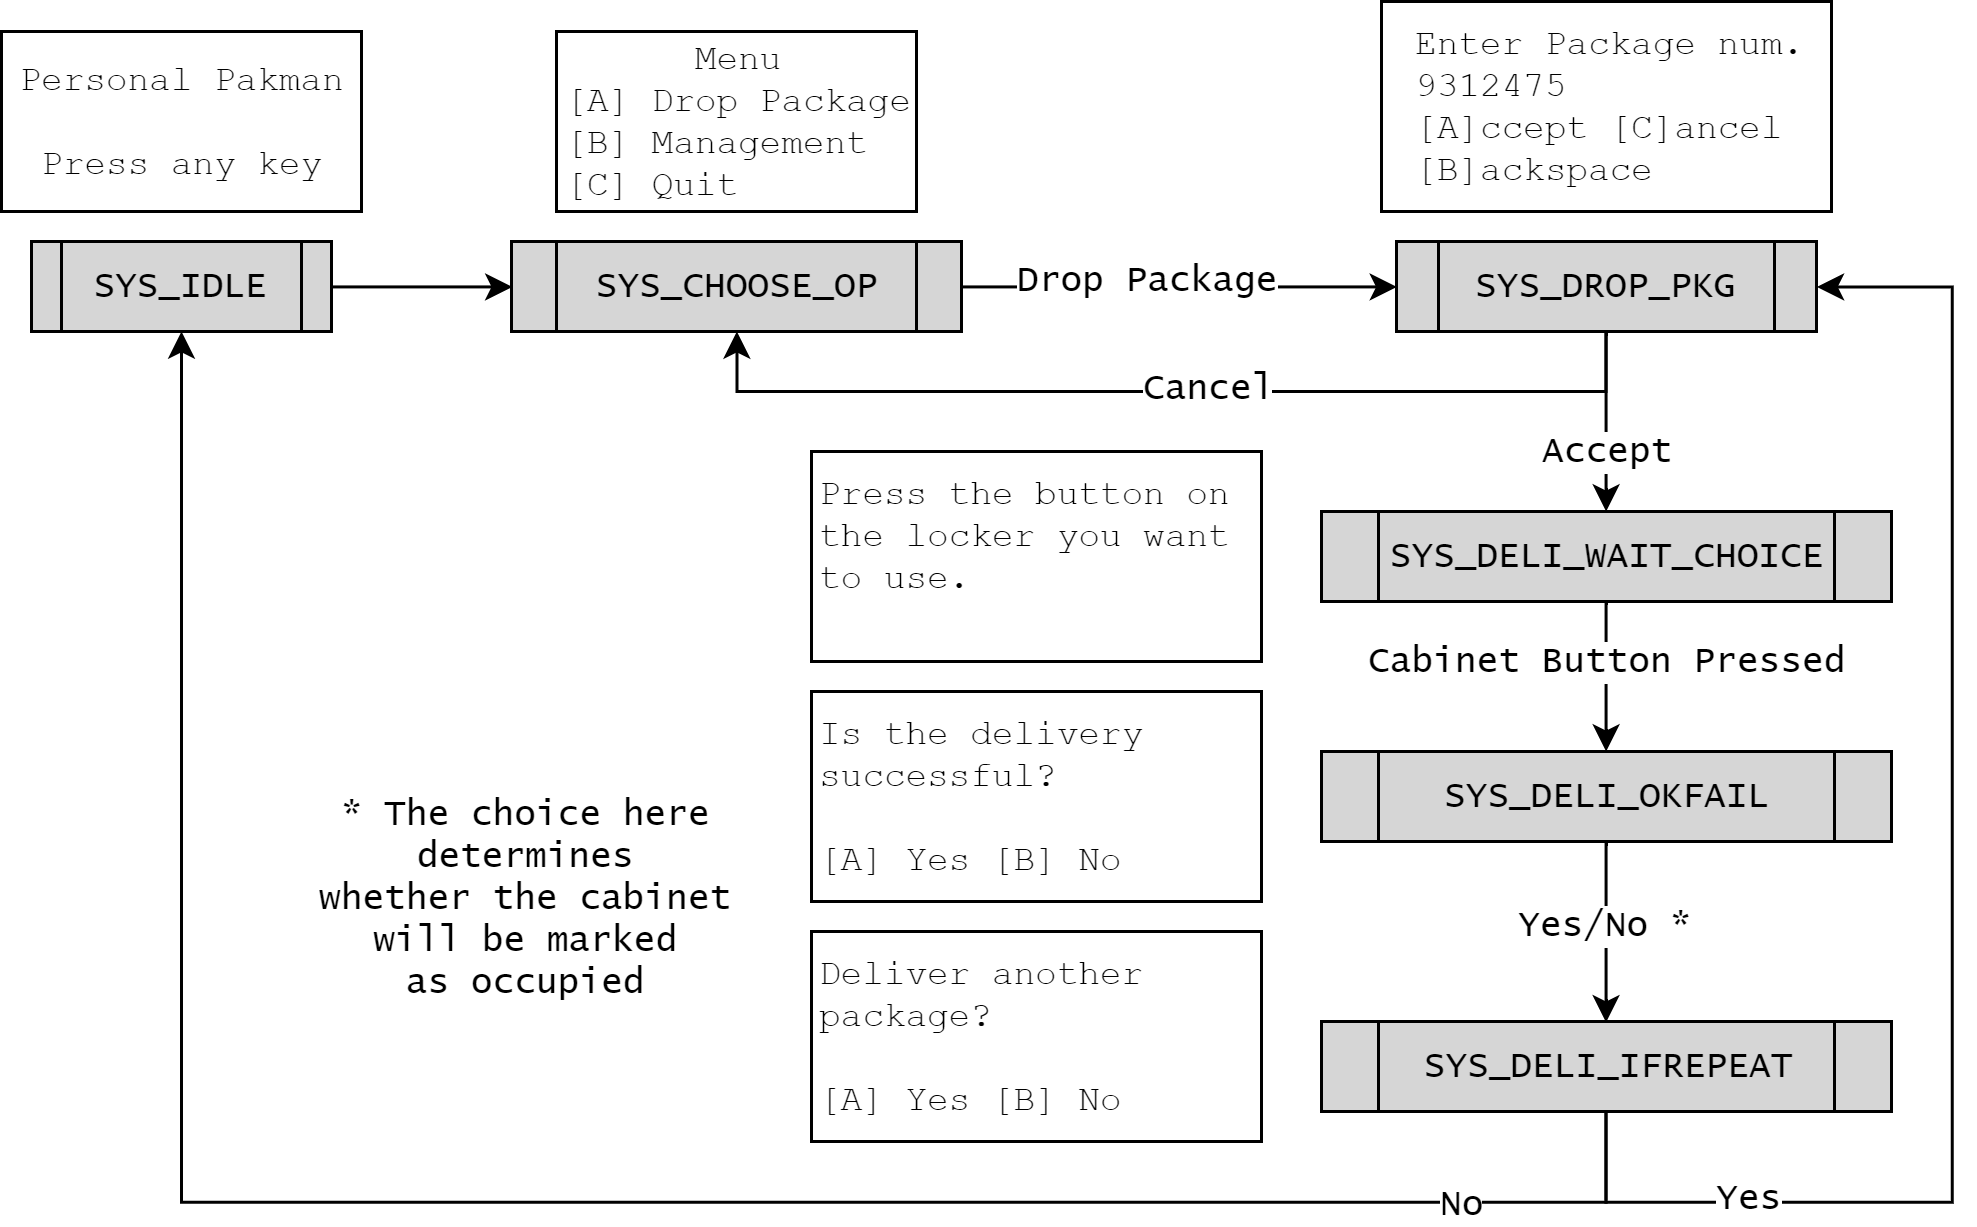
\includegraphics[width=\columnwidth]{pkg_logic.png}
\caption{Main Controller State diagram and screen outputs for delivering a package}
\end{figure}
\begin{figure}
\centering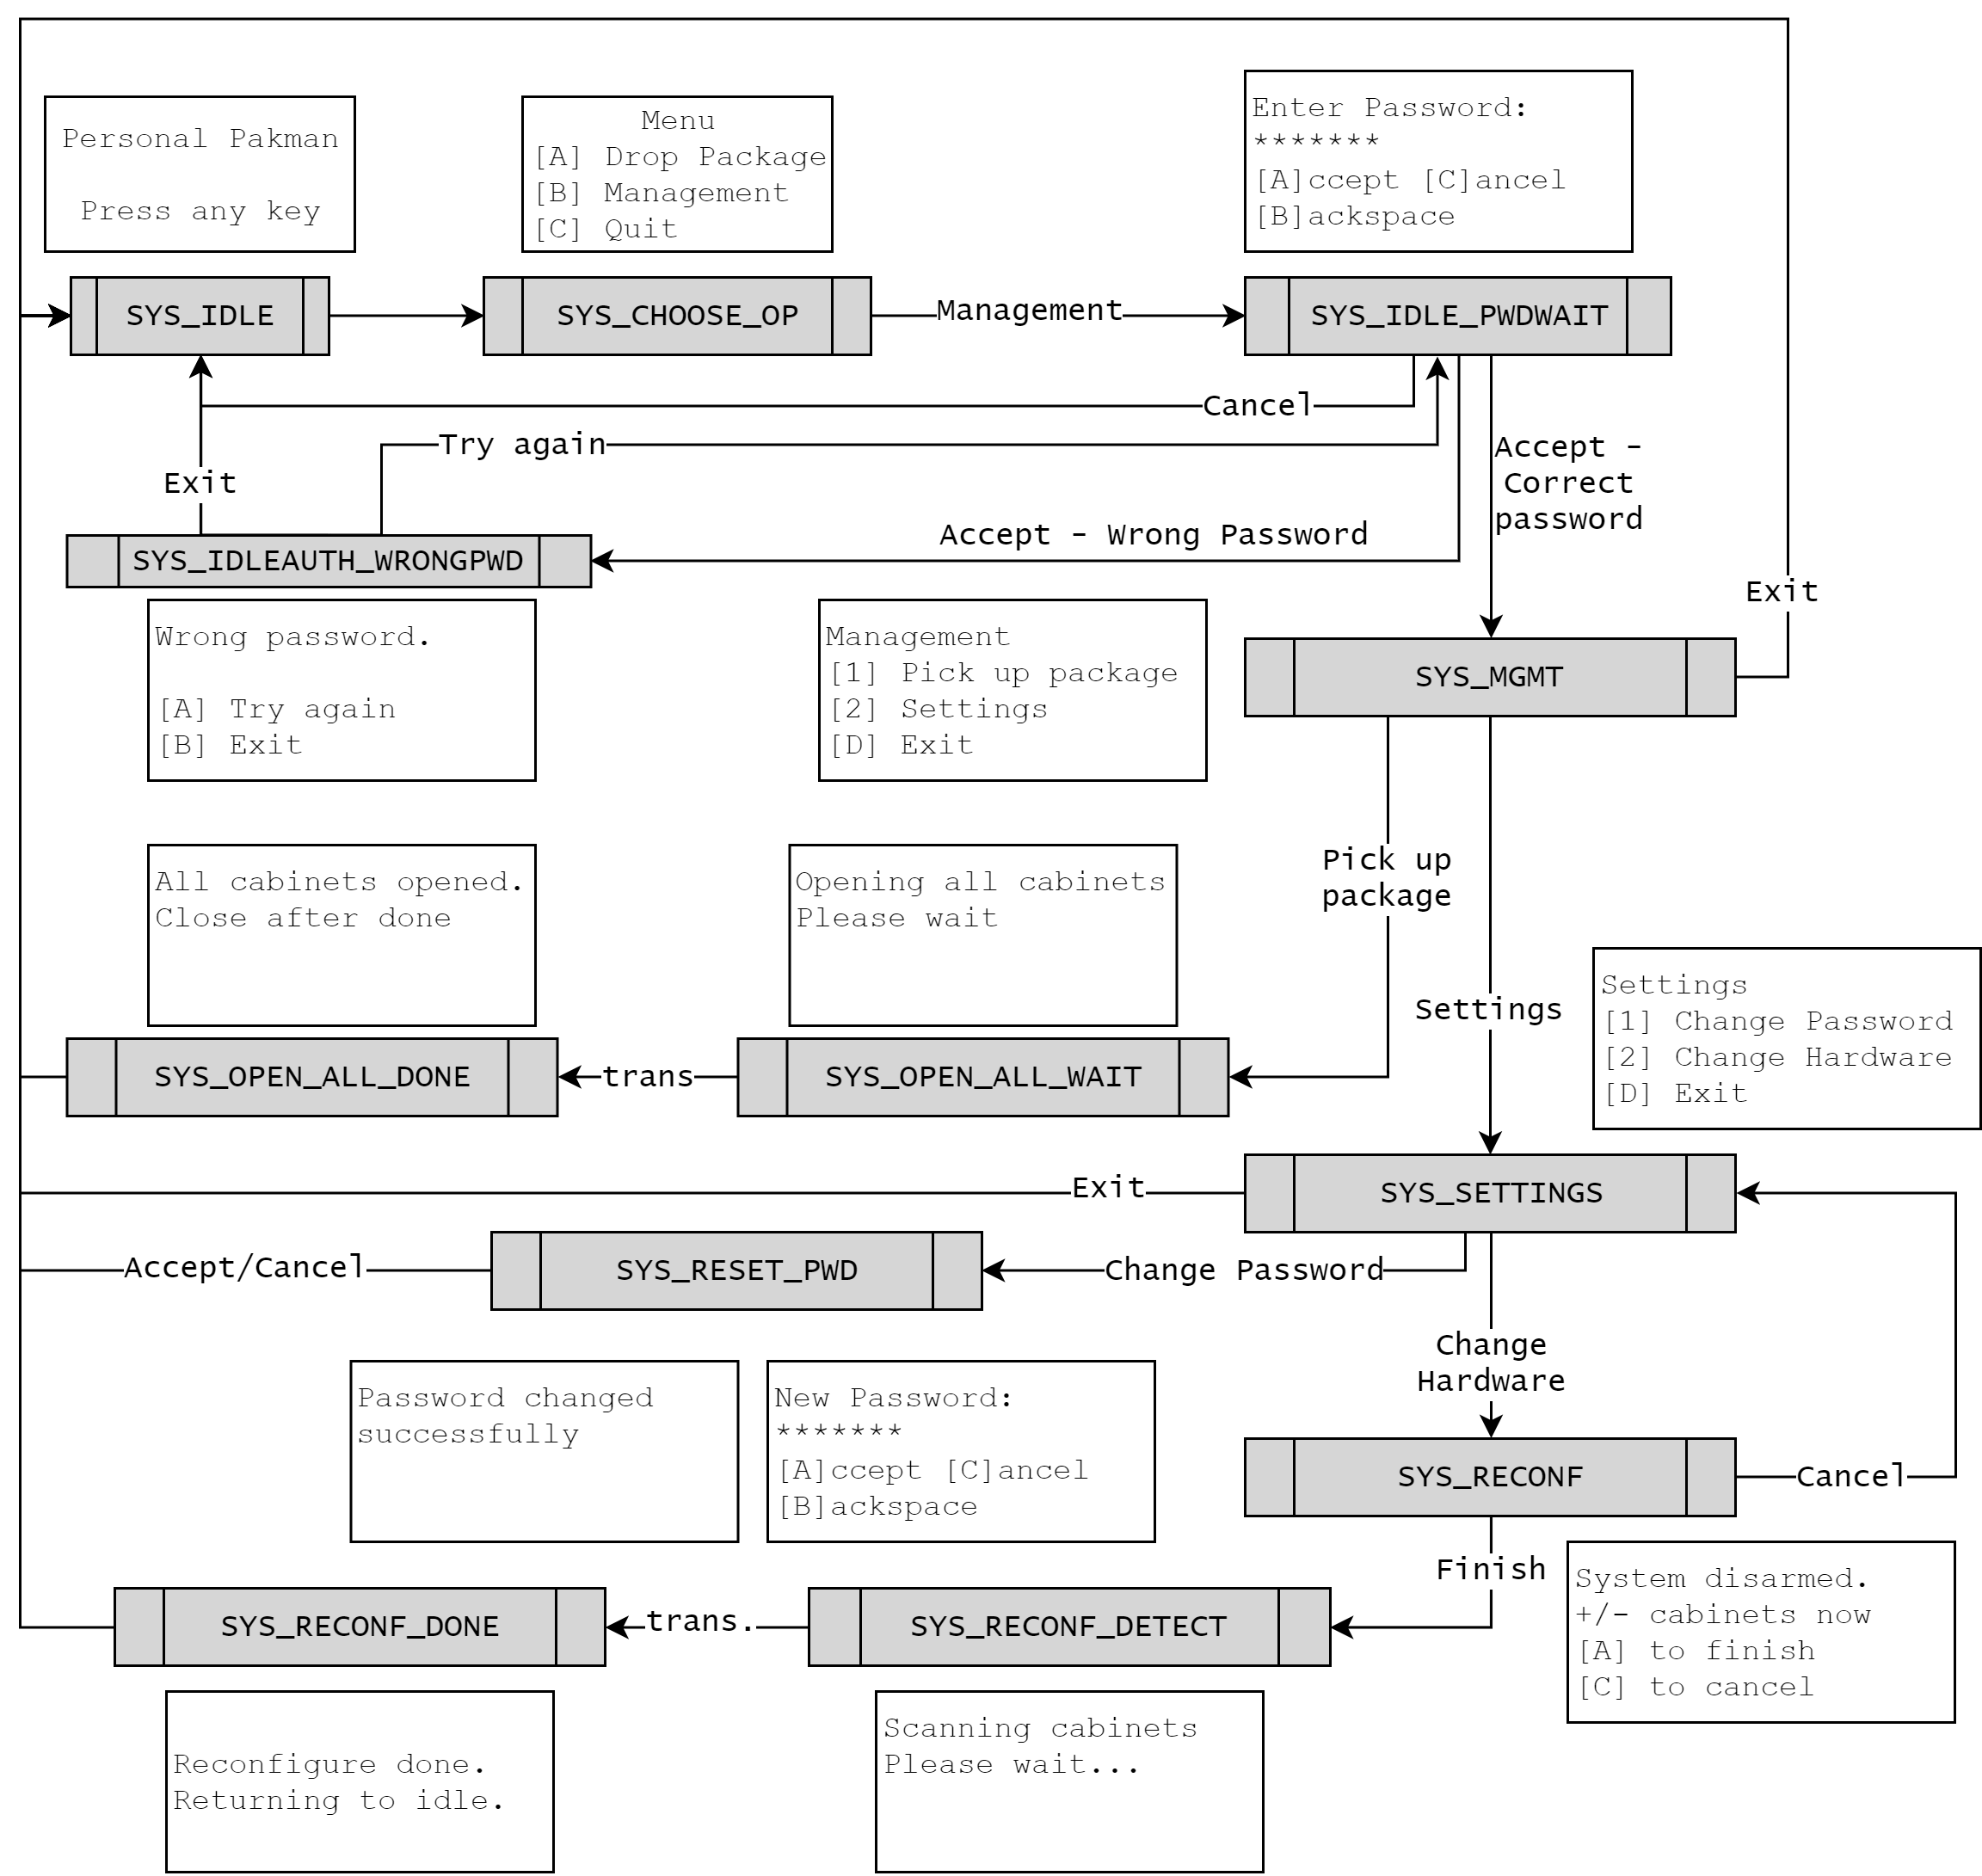
\includegraphics[width=\columnwidth]{pkg_mgmt.png}
\caption{Main Controller State diagram and screen outputs for system management}
\end{figure}
\section{Sub Controller Firmware}
\par The software for the sub-controllers are very simple. For the Arduinos, they can just use the Wire.h library to answer queries and execute commands from the central controller. Specific codes are used for transmission on the wire so each command or query will not exceed two bytes, eliminating the need for bandwidth and improves latency.
\par There's a shortcoming though: Slave address have to be pre-defined in the slave side of protocol, which means that we have to define different slave addresses in the program for each sub-controller manually. One way of solving this is to add a coding switch and tell the users to assign different patterns to each controller. There is another way complicated solution though, which I'll talk about in the "Future Development" chapter.
\section{Future Development}
\par The current project is a minimalist implementation of my idea, using the cheapest hardware to reach the basic goal. For this product to thrive in the modern world, I've got some development paths in my mind.
\par 1. Internet capabilities. For now, the cabinet cannot notify the user of a delivered package, nor can it fetch package data from the Internet. Connecting the controller to the Internet will allow it to automatically fetch data from various sites, provide web management interface, and send push notifications to the user. The controller I'm using have an Ethernet interface, but it does not have TCP/IP stack, not to say Linux. Using something else as the central processor, such as a Raspberry Pi, will allow these functionalities.
\par 2. Barcode Scanner. This feature was included when the project was proposed at the beginning, but then set aside for the difficulty of implementation. The USB Library provided by the toolchain have difficulty recognizing the barcode scanner. With more development effort or a more advanced platform (such as Raspberry Pis, as mentioned above), this will be less of a hassle.
\section{Conclusion}
\par In this project, I've built a package locker with decent functionality. It is able to store and handle packages for a single user, and provides a basic management interface. Given team and funding, this project can be expanded into a commercially viable product.
\section{Appendix}
\begin{itemize}
\item Code for this project can be found at: \texttt{https://github.com/Metric-Void/PakMan-Main}
\end{itemize}
\end{document} 